\subsection{Basis idee}
Het spel bestaat uit twee teams met een corresponderend hoofdgebouw voor elk team. Een team heeft minstens \'e\'en speler. Doel van het spel is om het commandocentrum van de tegenstander te vernietigen. De spelers behoren tot precies \'e\'en van de twee teams en hebben lasergeweren om de tegenstanders dood te schieten en torens aan te vallen. Torens kunnen door spelers worden neergezet op de map. Deze torens kosten goud om te bouwen. De spelers verdienen goud in een gezamenlijke kas door mijnen te bouwen over delfplaatsen. Verder kan goud worden verdiend door tegenstanders te doden en hun torens te vernietigen. Als een speler dood gaat of een toren kapot gaat, zal deze een muntje droppen dat vervolgens door alle spelers kan worden opgepakt.

\subsection{Terrein}
Het terrein kan in wezen allerlei vormen hebben, voorwaarde is dat het een eerlijk terrein is voor beide teams, een team mag dus geen voordeel hebben dankzij de kaart. De kaart heeft een rechthoekige vorm. Een goede manier waarop dit te verhinderen is, is door het terrein symmetrisch te maken. Op het terrein zijn twee commandocentrum geplaatst, voor beide teams een commandocentrum. Het kan gewenst zijn dat elk team bij de start van het spel ook al een aantal extra torens heeft ter bescherming van het commandocentrum. Over het terrein zijn een aantal delfplaatsen verdeeld. Deze zijn eerlijk verdeeld over de kaart. Andere obstakels mogen aanwezig zijn, maar zijn niet noodzakelijkerwijs aanwezig.

\begin{figure}
\center
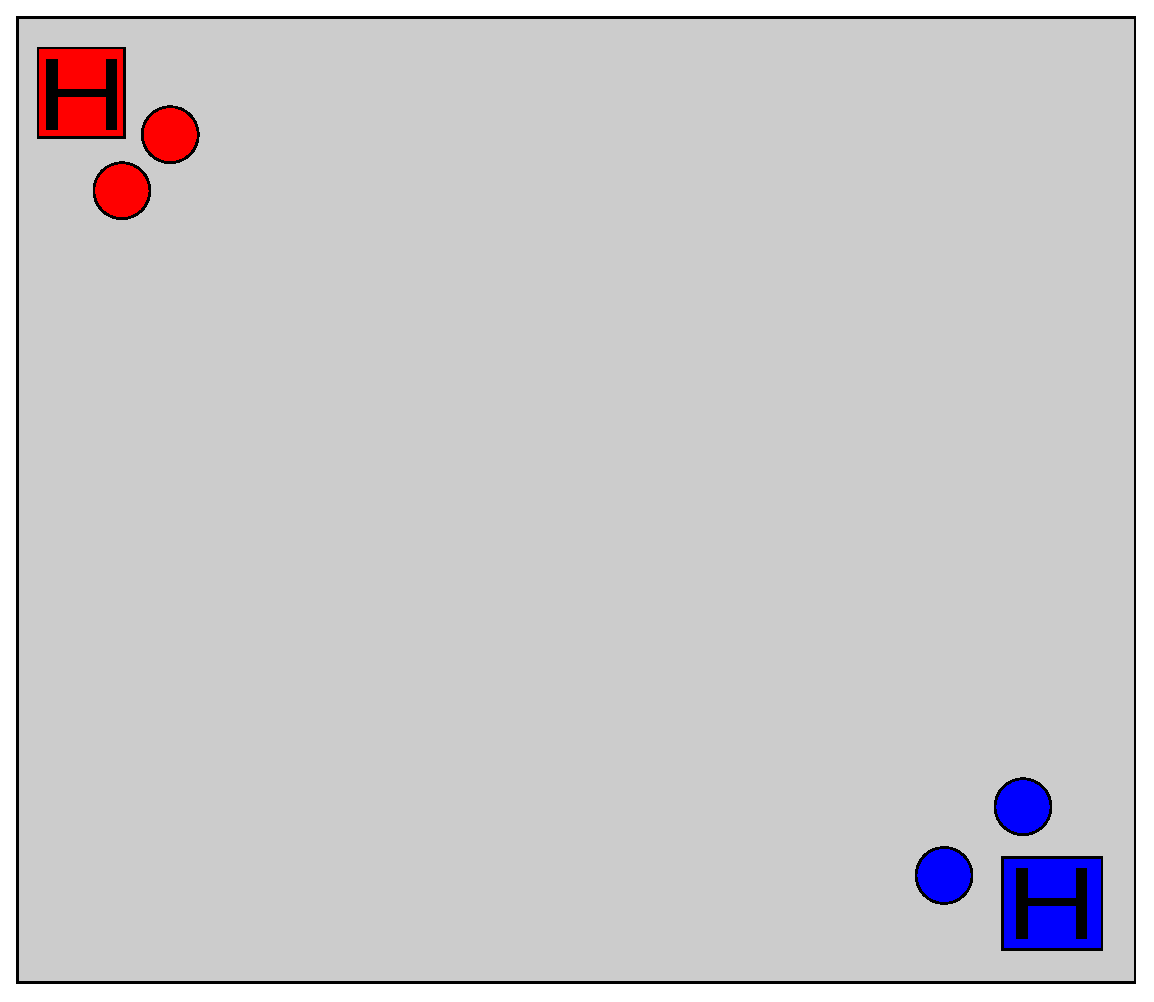
\includegraphics[width = 10cm]{Map1.eps}
\caption{Mogelijke kaart}
\label{fig:hist}
\end{figure}

\begin{figure}
\center
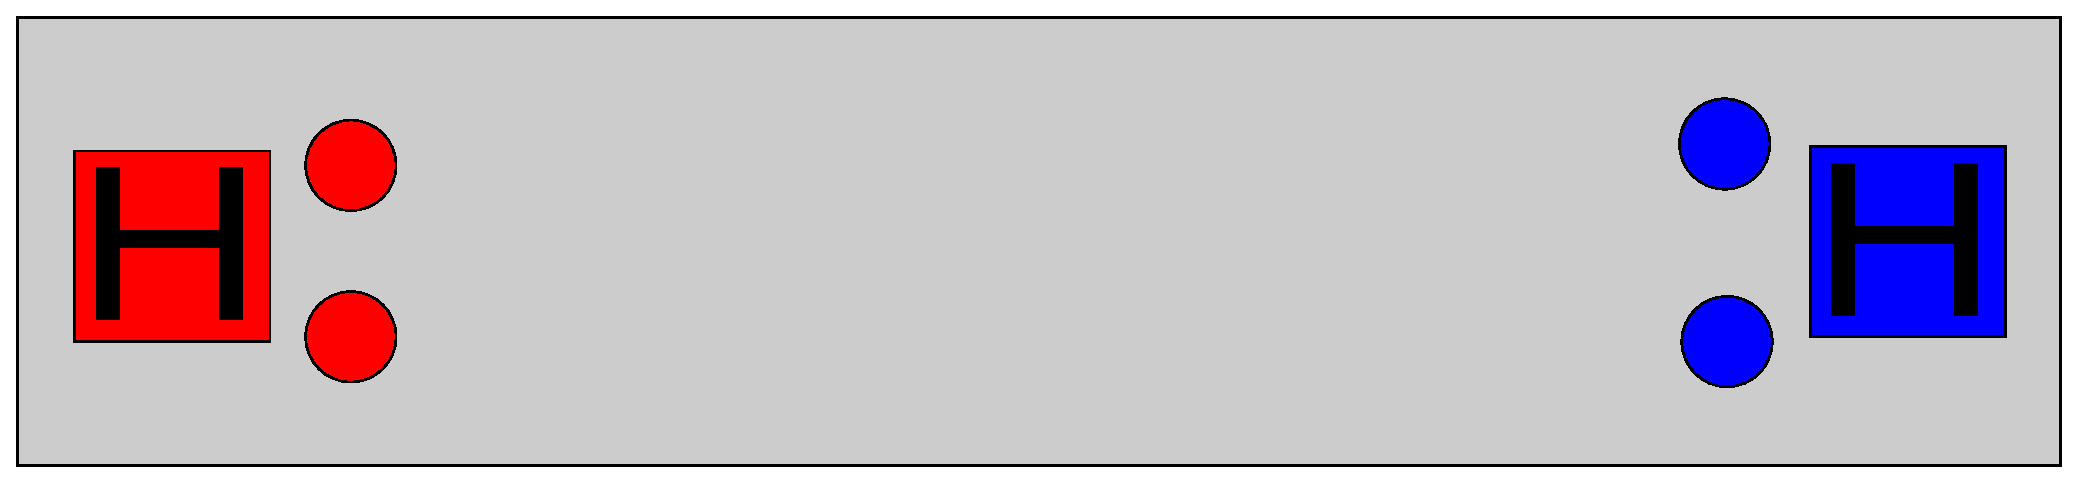
\includegraphics[width = 10cm]{Map2.eps}
\caption{Mogelijke kaart}
\label{fig:hist}
\end{figure}

\subsection{Spelers}
Een speler behoort tot een van beide teams, dit wordt duidelijk gemaakt door het kleuren schema van de speler. De speler heeft een lasergeweer waarmee hij op andere spelers en torens kan schieten om deze te vernietigen. Als een speler schiet, dan wordt geschoten in de huidige kijkrichting van de robot. Bij het begin van het spel heeft de robot nog een volledig harnas. Zodra de speler wordt geraakt, wordt de conditie van het harnas slechter. Het is echter niet mogelijk dat een speler het harnas van een andere speler uit hetzelfde team beschadigt.

De conditie van het harnas kan op geen enkele andere dan de hierboven beschreven manier veranderen. Een speler gaat dood als zijn harnas kapot is. In dat geval zal hij na een bepaalde hoeveelheid tijd terugkeren bij het hoofdgebouw met een volledig harnas. Ook kan een speler gebouwen bouwen, hiervoor gebruikt hij goud uit de kas van het team. De spelers kunnen op het grondvlak bewegen met een vaste snelheid in elke richting. De enige voorwaarde hierbij is dat de spelers op de kaart blijven en niet door een gebouw lopen. Het is dus wel mogelijk dat spelers door elkaar heen kunnen lopen. De spelers besturen hun karakter in een zogenaamde \emph{third person view}.

\subsection{Gebouwen}
Er zijn drie soorten gebouwen: Torens (gebouwen die op spelers en andere gebouwen in hun bereik kunnen schieten), mijnen (gebouwen die over een delfplaats kunnen worden gebouwd om de inkomsten van jouw team te vergroten) en een commandocentrum (het belangrijkste gebouw voor het team, als dit gebouw kapot is, heeft het bijbehorende team verloren). Alle gebouwen behoren tot een van beide teams, dit wordt duidelijk gemaakt door middel van het kleuren schema van het gebouw.

\subsection{Verzamelbare voorwerpen}
Er is maar \'e\'en verzamelbaar voorwerp: een muntje. Een muntje wordt achtergelaten door spelers die dood gaan en torens die worden vernietigd. Een muntje heeft een bepaalde waarde in goud. De waarde van het muntje is proportioneel aan de gezamenlijke kas van het team waarvan de speler is doodgegaan. Als een toren is vernietigd, dan is de waarde van het muntje proportioneel aan de kosten van de toren. De waarde van het muntje moet echter altijd kleiner zijn dan de kosten van de toren. Gedurende een spel moeten deze proporties vast zijn.

Als een speler doodgaat, wordt bovendien nog de waarde van het muntje afgetrokken van de gezamenlijke kas van die speler. Een muntje kan vervolgens opgepakt worden door alle spelers. De waarde van het muntje zal dan toegevoegd worden aan de kas van het bijbehorende team.

\subsection{Optioneel}
We hebben ook een aantal plannen voor uitbreiding van het spel, vooral om het uitgebreider te maken en leuker om te spelen. De volgende idee\"en staan op ons lijstje:
\begin{itemize}
  \item Plattegrond, zodat spelers een globaal overzicht krijgen van wat er in de arena gebeurt.
  \item Muren, als een extra type gebouw. Onze bedoeling hierbij is dat deze muren relatief goedkoop zijn om te bouwen. Dit geeft een team meer opties om hun commandocentrum of delfplaatsen te beschermen. Bovendien geeft het de extra mogelijkheid om een veilige plek te cre\"eren, waarvandaan tegenstanders aangevallen kunnen worden.
  \item Werkers, dit zijn computergestuurde robots. Zodra een speler daartoe opdracht geeft, komen werkers uit het commandocentrum van het bijbehorende team om een gebouw neer te zetten. Dit vervangt de oude mogelijkheid van spelers om te bouwen. Een gevolg van deze aanpassing is dat het langer duurt om een gebouw te bouwen als de afstand van de bouwplaats tot het commandocentrum groter is. Bovendien wordt het mogelijk om het bouwen van het andere team te vertragen door de werkers uit te schakelen.
  \item Infanterie, ook dit zijn computergestuurde robots. Deze kunnen door spelers worden gekocht, vanaf het commandocentrum lopen ze naar gebouwen van het andere team om deze gebouwen aan te vallen.
  \item Ontwikkelingen, de spelers krijgen ontwikkelingspunten tijdens het spel. Deze kunnen worden verdiend door het uitschakelen van spelers, werkers, infanterie en het vernietigen van gebouwen. Hiermee kunnen de spelers bijvoorbeeld de eigenschappen van hun robot verbeteren, zoals de snelheid van lopen en hoe sterk het harnas is. Ook is het mogelijk om sterkere wapens te kopen.
% Harnas opladen
\end{itemize} 